% ============================================================================
% หน้าปกคู่มือวิจัยฉบับสมบูรณ์ (RBRU Masterclass Academic Cover)
% โครงการ: SoilpHTxAI - มหาวิทยาลัยราชภัฏรำไพพรรณี
% ============================================================================

\begin{titlepage}
\thispagestyle{empty}
\begin{tikzpicture}[remember picture, overlay]
    % Background Gradient (Dark Navy to Midnight Blue)
    \fill[left color=rbruNavy!98!black, right color=rbruBlue!90!black] 
        (current page.south west) rectangle (current page.north east);
    
    % Top Gold Accent Lines
    \draw[line width=3pt, color=rbruGold] ($(current page.north west)+(25mm,-18mm)$) -- ($(current page.north east)+(-20mm,-18mm)$);
    \draw[line width=1pt, color=rbruGold!50] ($(current page.north west)+(25mm,-20mm)$) -- ($(current page.north east)+(-20mm,-20mm)$);
    
    % Header Banner (ลบคำว่า "รายงานและ" ออก)
    \node[anchor=north west, text width=155mm] at ($(current page.north west)+(25mm,-25mm)$) {
        {\fontsize{13}{16}\selectfont\bfseries\color{rbruGold} คู่มือวิจัยฉบับสมบูรณ์ (Comprehensive Research Monograph \& System Manual)\par}
        \vspace{1.5mm}
        {\fontsize{10.5}{13}\selectfont\color{white!80} ทุนอุดหนุนการวิจัยและนวัตกรรม มหาวิทยาลัยราชภัฏรำไพพรรณี ประจำปีงบประมาณ พ.ศ. 2569\par}
    };
    
    % Main Title Box (ตัดคำต่อเนื่อง ไม่ฉีกคำ กระชับและสละสลวย)
    \node[anchor=north, text width=160mm] at ($(current page.north)+(2.5mm,-48mm)$) {
        \begin{center}
            {\fontsize{23}{31}\selectfont\bfseries\color{white}
            การพัฒนาต้นแบบเครื่องวัดค่า pH ดินภาคสนามความแม่นยำสูง\\
            ด้วยการชดเชยอุณหภูมิอัจฉริยะโดยโครงข่ายประสาทเทียม\par}
            \vspace{3.5mm}
            {\color{rbruGold}\rule{0.65\textwidth}{1.8pt}\par}
            \vspace{3mm}
            {\fontsize{11.5}{15}\selectfont\itshape\color{white!90}
            Development of High-Accuracy Field-Portable Soil pH Meter Prototype\\
            with Intelligent Temperature Compensation Using Neural Networks\par}
            \vspace{2.5mm}
            {\fontsize{13}{16}\selectfont\bfseries\color{rbruCyan} [ SoilpHTxAI Edge AI System ]\par}
        \end{center}
    };

    % Real Smartphone Hero Device Mockup (ภาพจริงของหน้า application ตรงกลางอย่างสง่างาม)
    \node[anchor=center] at ($(current page.center)+(2.5mm,-18mm)$) {
        \begin{tikzpicture}
            % Ambient Backlight Glow
            % Smartphone ambient aura
            
            % Outer Gold/Titanium Smartphone Chassis with Drop Shadow
            \draw[rounded corners=22pt, fill=black!92, draw=rbruGold, line width=2.6pt, drop shadow={opacity=0.75, shadow xshift=6pt, shadow yshift=-7pt}] (-2.85,-6.05) rectangle (2.85,6.05);
            
            % Inner Bezel
            \draw[rounded corners=18pt, fill=black, line width=0.8pt, draw=black] (-2.7,-5.9) rectangle (2.7,5.9);
            
            % Real Application Screenshot Clipped into Display
            \begin{scope}
                \clip[rounded corners=16pt] (-2.65,-5.85) rectangle (2.65,5.85);
                \node at (0,0) {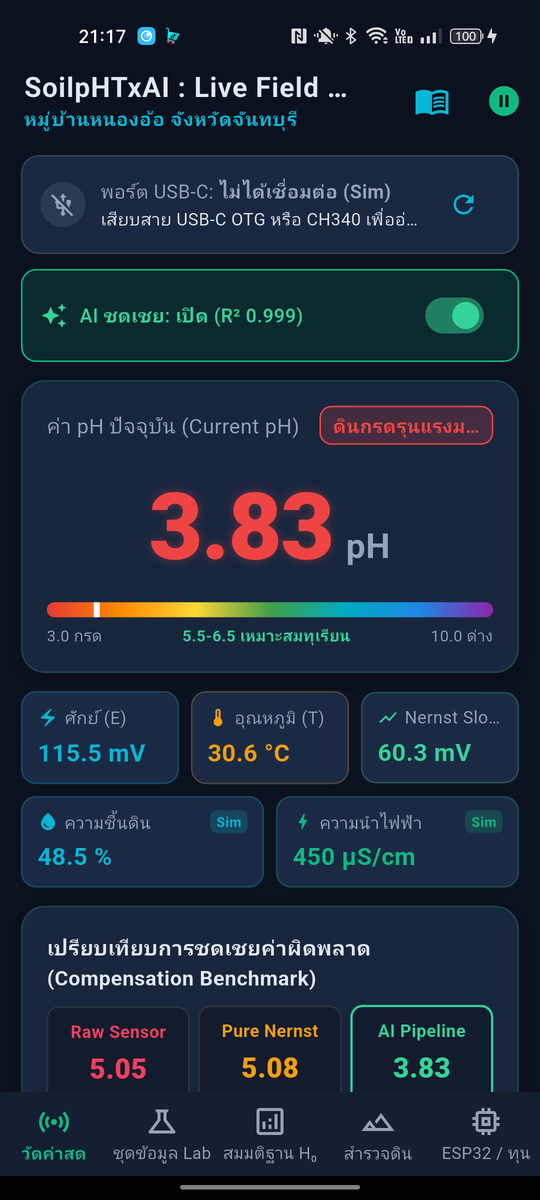
\includegraphics[width=5.3cm, height=11.7cm]{figures/app_screen_usb_opt.png}};
            \end{scope}
            
            % Dynamic Island / Camera Punch Hole
            \draw[rounded corners=4pt, fill=black, draw=white!15, line width=0.4pt] (-0.85,5.48) rectangle (0.85,5.74);
            \fill[blue!40!black] (0.4,5.61) circle (1.6pt);
            
            % Subtle Glass Glare Reflection
            \begin{scope}
                \clip[rounded corners=16pt] (-2.65,-5.85) rectangle (2.65,5.85);
                \fill[white, opacity=0.07] (-4,7) -- (5,7) -- (-1,-7) -- (-4,-7) -- cycle;
            \end{scope}
            
            % High-Tech Hardware Status Badge
            \node[anchor=south, fill=rbruNavy!95!black, draw=rbruEmerald, line width=1pt, rounded corners=4pt, inner sep=4pt] at (0,-6.7) {
                {\fontsize{8.5}{11}\selectfont\bfseries\color{white} \textcolor{rbruEmerald}{\Large$\bullet$} Live Telemetry: USB-C Modbus RTU \quad \textcolor{rbruGold}{|} \quad Pure Dart Edge AI}
            };
        \end{tikzpicture}
    };

    % Publisher & Attribution Footer (ลบคำว่า "จัดทำขึ้นโดย" ออก และตัดกล่องคณะผู้วิจัยออกตามสั่ง)
    \node[anchor=south, text width=160mm] at ($(current page.south)+(2.5mm,16mm)$) {
        \begin{center}
            {\fontsize{13}{17}\selectfont\bfseries\color{white} ผศ.ดร.ชีวะ ทัศนา\par}
            \vspace{1.5mm}
            {\fontsize{10}{13}\selectfont\color{white!85} หน่วยวิจัยปัญญาประดิษฐ์เพื่อเกษตรดิจิทัล คณะวิทยาศาสตร์และเทคโนโลยี มหาวิทยาลัยราชภัฏรำไพพรรณี\par}
            \vspace{1mm}
            {\fontsize{8.5}{11}\selectfont\color{rbruGold!80} ลิขสิทธิ์ของมหาวิทยาลัยราชภัฏรำไพพรรณี ประจำปีงบประมาณ พ.ศ. 2569\par}
        \end{center}
    };
\end{tikzpicture}
\end{titlepage}
